\documentclass[11pt,titlepage]{article}
\usepackage{fullpage}
\usepackage{amsmath}
\usepackage{amssymb}
\usepackage{color}
\usepackage{graphicx}
\graphicspath{ {images/} }
\usepackage{tikz}
\usetikzlibrary{shapes,arrows,positioning,calc}
\usepackage{float}
\restylefloat{table}
\usepackage{array}
\tikzset{
    block/.style = {draw, fill=white, rectangle, minimum height=3em, minimum width=3em},
    sum/.style = {draw, fill=white, circle, node distance=1cm},
    input/.style = {draw=none},
    output/.style = {draw=none},
    coord/.style = {coordinate}
}

\author{Rane Brown \\ Kate Schneider}
\title{ECEN 4638: Lab X.1PI}
\date{\today}

\begin{document}
\maketitle
\tableofcontents
\listoffigures
\newpage

\section{Description}
    This lab will further explore the Torsional Disc System using Proportional-Integral control, with the goal of designing a PI-based cruise control system that works well for inertia changes of $\pm10\%$. The controller is then tested on two different Torsional Disc apparatuses to evaluate the design for robustness. The system setup will be similar to what was used in labX.1P; only the bottom disc of the TDS will be used and the four weights will be set at a radius of 7.5cm.

\section{System Model}
   As in labX.1P, the Torsional Disc system can be modeled as an LTI system, with the below equation
    \begin{equation} \label{eq:lti}
        J\dot{\omega}+c\omega=k_hu
    \end{equation}
    Where $J=\mbox{ total system inertia}$, $\omega=\mbox{ velocity rad/sec}$, $c=\mbox{ system drag}$, $k_h=\mbox{ hardware gain}$, $u=\mbox{ reference}$.
    
    
    \subsection{Calculated Parameters}
        During labX.1P, each team calculated parameters $c$ and $k_h$ for one torsional disc system based on its experimental data. These parameters are listed in the table below.

    
            \begin{table}[h!]
            \centering
            \begin{tabular}{|m{4cm}|m{3cm}|m{3cm}|} 
                \hline
                System & $c$ &$k_h$ \\ 
                \hline
                1 &  0.0082 & 0.3577\\
                \hline
                \textbf{1} & \textbf{0.0079} & \textbf{0.3598}\\
                \hline
                2 & 0.0078 & 0.15\\
                \hline
                2 & 0.0081 & 0.376\\
                \hline
                3 & 0.0110 & 0.387\\
                \hline
                3 & 0.010 & 0.0084\\
                \hline
                4 & 0.0111 & 0.0084\\
                \hline
                4 & 0.0184 & 0.387\\
                \hline
            \end{tabular}
            \caption{Torsional Disc System Parameters} \label{table:TDS_param}
        \end{table}
        
        For a radius of 7.5 cm, the calculated total system inertia $J$ is 0.0128 $kg m^2$.
        
        For this experiment, our cruise control system was designed using the calculated parameters from Torsional Disc System 1 (in bold in the above table), and the PI controller was tested on TDS systems 1 and 4.

    \subsection{Transfer Functions}
    
	\begin{figure}[H]
	\centering
	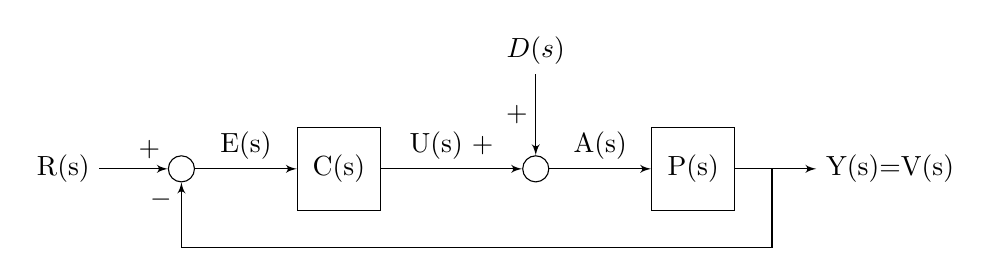
\begin{tikzpicture}[auto, node distance=2cm,>=latex']
		\node [input, name=rinput] (rinput) {R(s)};
		\node [sum, right of=rinput, node distance=1.5cm] (sum1) {};
		\node [coord, below of=sum1, node distance=1cm] (fdbk1) {};
		\node [block, right of=sum1] (controller) {C(s)};
		\node [sum, right of=controller, node distance=2.5cm] (sum2) {};
		\node [block, right of=sum2, node distance=2cm] (plant) {P(s)};
		\node [coord, right of=plant, node distance=1cm] (fdbk2) {};
		\node [coord, below of=fdbk2, node distance=1cm] (fdbk3) {};
		\node [input, above of=sum2, node distance=1.5cm] (disturbance) {$D(s)$};
		\node [output, right of=plant, node distance=2.5cm] (output) {Y(s)=V(s)};
		\draw [->] (rinput) -- node[xshift=.2cm]{$+$} (sum1);
		\draw [->] (disturbance) -- node[xshift=-.5cm]{$+$} (sum2);
		\draw [->] (sum1) --node {E(s)} (controller);
		\draw [->] (controller) -- node{U(s) $+$} (sum2);
		\draw [->] (sum2) -- node{A(s)} (plant);
		\draw [->] (plant) -- node {}(output);
		\draw [-] (fdbk2) -- (fdbk3);
		\draw [-] (fdbk3) -- (fdbk1);
		\draw [->] (fdbk1) -- node[yshift=.2cm]{$-$} (sum1);
	    \end{tikzpicture}
	\caption{Cruise Control Feedback System} \label{fig:block}
	\end{figure}
    
    	From our LTI model, we see that the system plant is modeled with the below equation.
 	\begin{equation} \label{eq:lti}
       		P(s)= \frac{k_h}{Js+c}e^{-T_ds}
    	\end{equation}
    Where $J=\mbox{ total system inertia}$, $c=\mbox{ system drag}$, $k_h=\mbox{ hardware gain}$, and $T_d=\mbox{ time delay}$.
    In this lab, we use a PI controller, $C(s)=\frac{k_I}{s}+k_p$. \\
    
    \textcolor{red}{include info from sheet on these and what they tell us!! Then add plots!!}
    There are multiple transfer functions which are of interest in our system. The first transfer function of interest is the closed-loop transfer function from reference input $R$ to output $Y$:
	\begin{equation}
		H_{yr}=\frac{Y}{R}=\frac{CP}{1+CP}=\frac{kk_I+kk_ps}{Js^2+(c+kk_p)s+kk_I}
	\end{equation}
	
	From the equation for $H_{yr}$, we can see that the DC gain of this transfer function is 1, as we would expect \textcolor{red}{because...}.
	
	Another transfer function of interest is the closed-loop transfer function from reference input $R(s)$ to controller output $U(s)$.
	\begin{align}
		H_{ur}&=\frac{U}{R}=\frac{C}{1+CP}=\frac{Jck_Ik_ps^3+Jk_Is^2+ck_Is}{Js^2+(c+kk_p)s+kk_I}
	\end{align}
	
	This transfer function has a DC gain of  $H_{ur}(0)=\frac{c}{k}$. This value represents the input that is needed to compensate parameter $c$ in steady state. 
		
	We can also look at the transfer function from the disturbance $D(s)$ to the output $Y(s)$, since again, rejecting disturbance input such as hills and bumps is important in a cruise control system.
	\begin{equation}
		H_{yd}=\frac{Y}{D}=\frac{\frac{k}{J}s}{s^2+(\frac{c}{J}+\frac{k_pk}{J}s)+\frac{k}{J}k_I}
	\end{equation}
	
	The final closed-loop transfer function of interest is $H_{ud}$, the transfer function from the disturbance $D(s)$ to the controller output $U(s)$. 
	\begin{equation}
		H_{ud}=\frac{-\frac{k}{J}(k_ps+k_I)}{s^2+(\frac{c}{J}-\frac{kk_p}{J})s+\frac{kk_I}{J}}
	\end{equation}	
		
	We will also examine the open-loop transfer function $L(s)=P(s)C(s)$, which will be useful in determining gain and phase margins of our system to ensure stability.
	
	\begin{equation}
		L(s)=P(s)C(s)=	\frac{k}{Js+c}(\frac{k_I}{s}+k_p)
		\end{equation}

\section{Matlab Analysis}
    \subsection{Time Domain}
	    Before implementing our PI controller on a physical TDS, we can formulate and test the design in Matlab to ensure the system meets certain time and frequency domain specifications. In the time domain, relevant specifications include rise time $t_r$, settling time $t_s$, and overshoot $M_p$. Choosing desired ranges for these parameters allows us to estimate $\zeta$ and $\omega_{n}$ for a simple second-order system of the form
	    
	    \begin{equation}
	    	\frac{K\omega_n^2}{s^2+2\zeta \omega_ns+\omega_{n}^2}
	    \end{equation}
	    
	    with the relationships 
	    \begin{equation}
	    	t_r = \frac{1.8}{\omega_n}, \hspace{1cm} t_s=\frac{4.6}{\zeta\omega_n},  \hspace{1cm}  M_p=e^{\frac{-\pi \zeta}{\sqrt{1-\zeta^2}}}
	    \end{equation}
    
    	However, when using these estimates, we must keep in mind that our PI controller also introduces an additional zero to the closed-loop transfer function $H_{yr}(s)$ which will affect the time domain response of our system. Most notably this zero will increase $M_p$ and decreasing $t_r$. Thus, design must aim for a larger $\zeta$, while $\omega_n$ can be decreased slightly and still meet rise time specifications. \\
    
    	If, for instance, we choose desired values of $t_r<1 sec$, $t_s < 5 sec$, and $M_p<10\%$, we can estimate suitable $\omega_n$ and $\zeta$ for $H_{yr}(s)$ by hand calculation, then model the system in Matlab. Iterating on the design in Matlab allows us to fine-tune the controller, which we can then evaluate on the physical system.\\
	\textcolor{red}{discuss/plot all the other transfer functions!!!}
	
	The specifications above results in the values $\omega_n = , \hspace{1cm} \zeta= $ which gives values $k_i= , k_p= $. This results in the system transfer function $H_{yr}(s) = $. The plot for $H_{yr}(s)$ is given below.
	
	\textcolor{red}{add plot here}
	
	From the above plot, we can see that the additional zero results in a greater overshoot and overall faster response. The plots of the other three transfer functions of interest are included below. \textcolor{red}{add other TF plots here}
	
	We can further refine our design in order to get a better time domain response from our system, now that we have observed the effect of the additional zero in Matlab simulations. \textcolor{red}{include one more iteration, with better params which worked for the exp sys.}
	
    \subsection{Frequency Domain}
    	In addition to time domain specifications, certain aspects of a system's frequency domain response are important to take into consideration to ensure the stability and good performance of that system. These values are the steady-state error, $e_{ss}$, the phase margin $PM$, the gain margin $GM$, and the bandwidth,, which gives us the system's half-power frequency. $e_{ss}$ and  $\omega_{BW}$ are important for system performance. $PM$, and $GM$ ensure stability of the system, with $45<PM<60$ an ideal region for the phase margin, $GM>__$ a good goal for gain margin. 
	
	We can plot the frequency response of our first system () and analyze the stability and performance of the system. Note that we have \\
	$PM=__$, $GM=__$, \omega_{BW}=_$, and $e_{ss}=__$. \textcolor{red}{discuss what these mean, then do an iteration using freq plots. FINALLY, put all of these together into a system that has good time and freq response characteristics in Matlab. Make sure for this system you plot several other transfer functions as well - use one that may have performed well on the TDS itself.}
	 
\section{Experimental Analysis}
    \subsection{Time Domain}

    \subsection{Frequency Domain}

\section{PI Controller Design}

\end{document}